% 封面字級只作用在該行，換段（\par）放在大括號外，行距才不會被放大

%%%%    中文封面
\begin{center}
\vspace*{1cm}

{\fontsize{12}{18}\selectfont （學校系所待填）專題報告}\par

\vspace*{3.5cm}

{\Huge\textbf{羽球比賽分析系統}}\par
{\Large\textbf{從羽球單打轉播影片自動產出逐拍資料}}\par

\vspace*{6cm}

{\fontsize{16}{24}\selectfont 作者}\par
\begin{tabular}{c}
（學號）（姓名）（電子郵件）\\
（學號）（姓名）（電子郵件）\\
（學號）（姓名）（電子郵件）
\end{tabular}\par

\vspace*{1.5cm}

{\fontsize{16}{24}\selectfont 指導教授：（待填）\hspace{0.5cm}博士}\par

\vspace*{2cm}

{\fontsize{12}{18}\selectfont 中　華　民　國　一　百　一　十　五　年　　月　　日}\par
\end{center}

\clearpage

%%%%    英文封面
\begin{center}
\vspace*{1cm}

{\fontsize{12}{18}\selectfont Project Report (department to be filled)}\par

\vspace*{3.5cm}

{\Huge\textbf{Badminton Analysis System}}\par
{\Large\textbf{Automatic Stroke-Level Data from Singles Broadcast Videos}}\par

\vspace*{3.5cm}

\textbf{Author}\par
\begin{tabular}{c}
(Student ID) (Name) (Email)\\
(Student ID) (Name) (Email)\\
(Student ID) (Name) (Email)
\end{tabular}\par

\vspace*{1.5cm}

{\fontsize{16}{24}\selectfont \textbf{Advisor}：Dr. (to be filled)}\par

\vspace*{2cm}

{\fontsize{12}{18}\selectfont 2026/\,\,/\,\,}\par
\end{center}

\clearpage

%%%%    專題分工及貢獻度說明
\begin{center}
{\fontsize{16}{24}\selectfont\textbf{專題分工及貢獻度說明}}\par
\vspace*{1cm}
\begin{tabular}[c]{|l|l|p{10cm}|l|}
  \hline
  編號 & 姓名 & 主要工作內容 & 專題貢獻度 \\
  \hline
  1 & （待填） & （待填） & \\
  \hline
  2 & （待填） & （待填） & \\
  \hline
  3 & （待填） & （待填） & \\
  \hline
\end{tabular}
\end{center}

\clearpage

%%%%    專案管理系統截圖（不編號、不列入圖目錄）
\begin{center}
{\fontsize{16}{24}\selectfont\textbf{專案管理系統截圖}}\par
\vspace*{1cm}
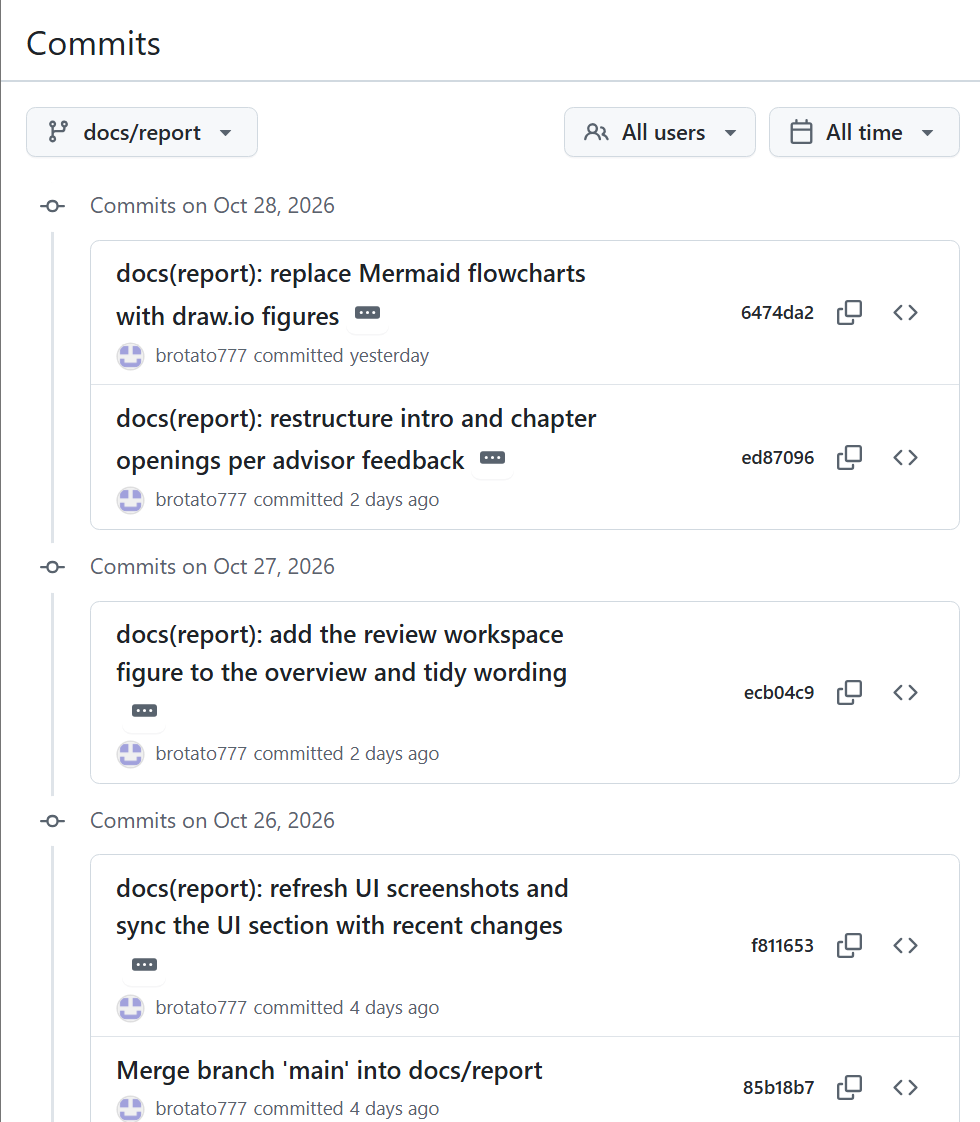
\includegraphics[width=0.45\linewidth]{project_management/github_commits_report.png}\hfill
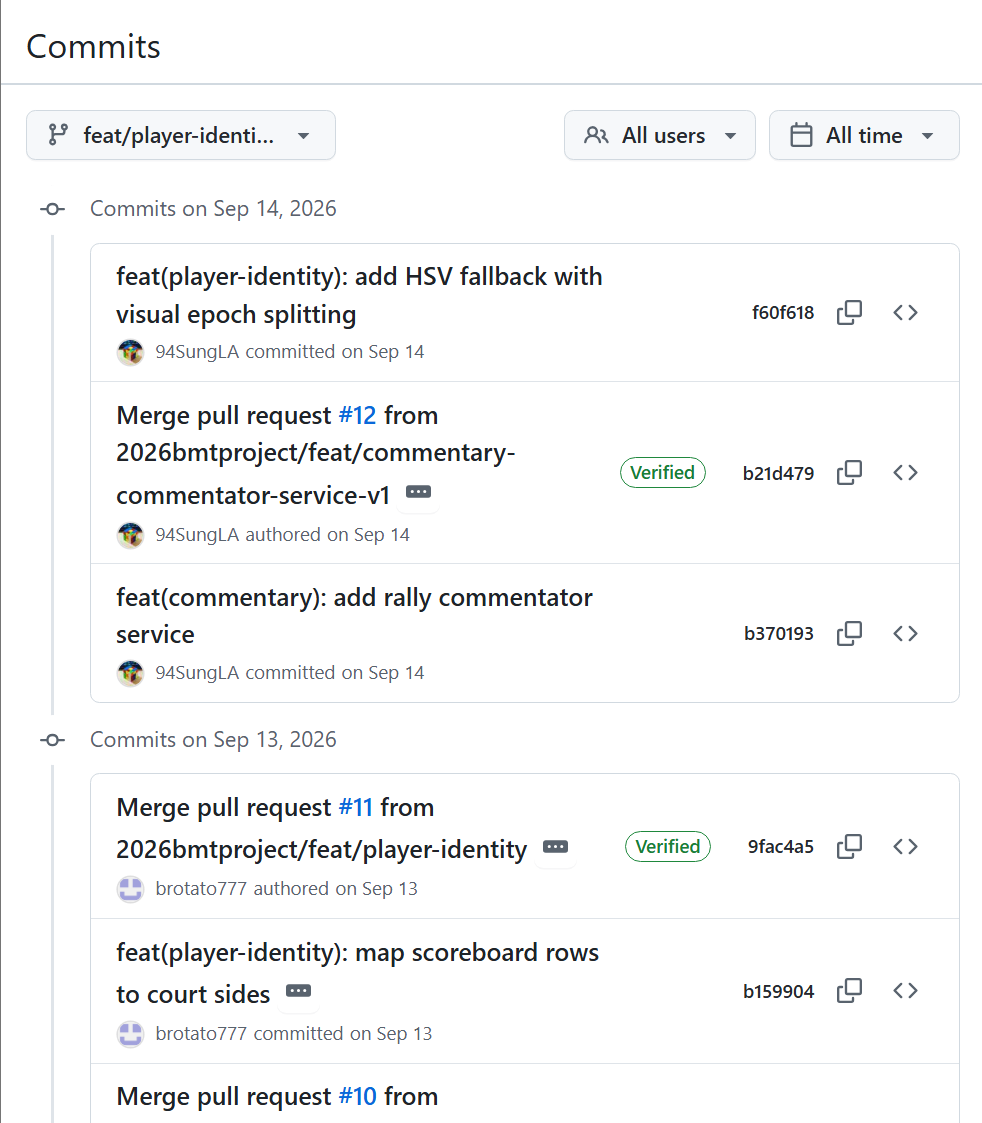
\includegraphics[width=0.45\linewidth]{project_management/github_commits_identity.png}\par
\vspace*{0.3cm}
GitHub 工作紀錄\par
\vspace*{1cm}
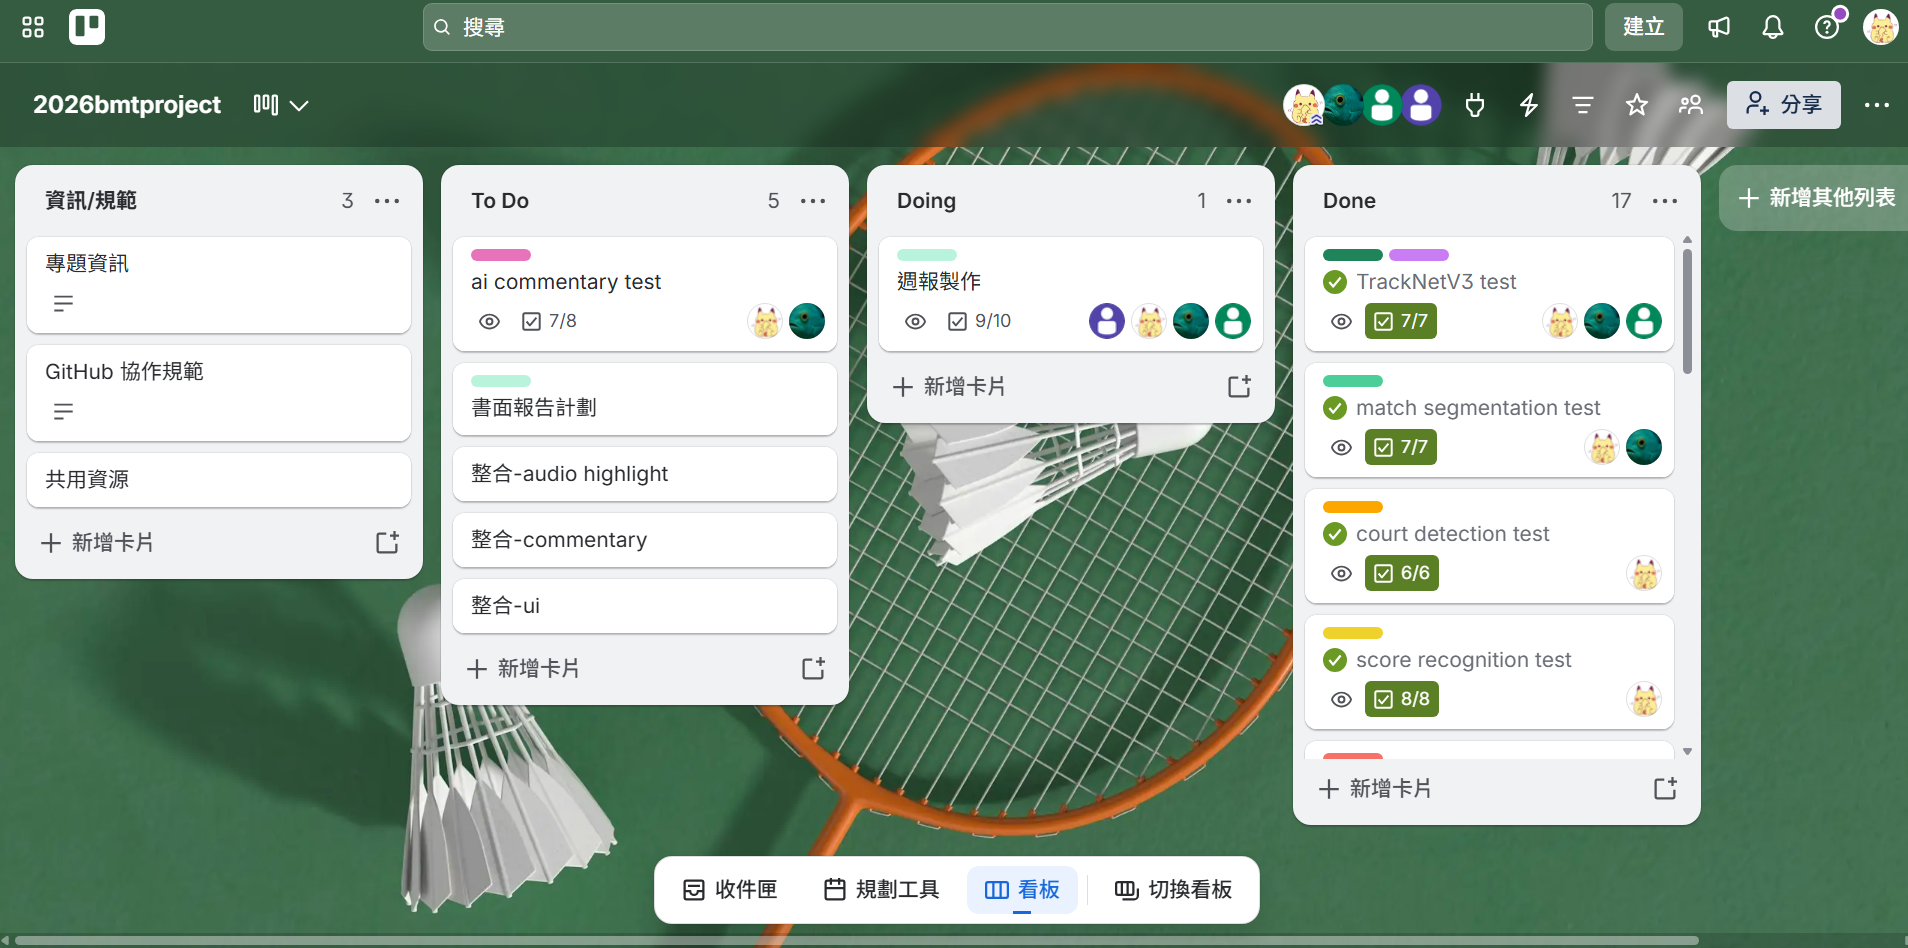
\includegraphics[width=\linewidth]{project_management/trello.png}\par
\vspace*{0.3cm}
Trello 工作紀錄\par
\end{center}

\clearpage
